\section{Introduction}

\subsection{Objectives}

\begin{itemize}
    \item Identify the image processing steps of a recipe such filtering, segmentation and binary processing.
    \item Manage records and table.
    \item Create a GA3 recipe for a given analysis problem.
    \item Batch process collection of files.
\end{itemize}

\subsection{General interface}

\paragraph{Preliminary steps}
Once the GA3 module opened, other windows cannot be opened, therefore
\begin{itemize}
    \item you will need to open the image you want to work with first,
    \item it is convenient to open the LUTs tools first (\keys{\ctrl+\Alt+L}).
\end{itemize}
To access the GA3 interface, you can either:
\begin{itemize}
    \item use the menu \menu{Image>New GA3 recipe\dots},
    \item use the menu \menu{Image>Analysis Explorer\dots} to open the analysis exporter and then click on \menu{Create New},
    \item right-click on the background of the interface, select \menu{Analysis Controls>Analysis Explorer} to open the analysis exporer and then click on \menu{Create New}.
\end{itemize}

\paragraph{Loading and saving recipes}

\begin{itemize}
    \item Use \menu{Save} or \menu{Save As} to save the recipe in the local database. It will be then listed in the Analyis Explorer.
    \item Use your name as a prefix so that we can contact you if the database needs to be cleared.
    \item Use \menu{Export} to export the recipe in a folder of your choice. This recipe can then be reloaded on another computer. It is good practice to have a copy of the recipes in that way.
    \item Use \menu{Import} to reload an exported recipe. 
\end{itemize}

\paragraph{Recipes}
\begin{figure}
    \centering \small
    \begin{tikzpicture}
        \node at (0,0) {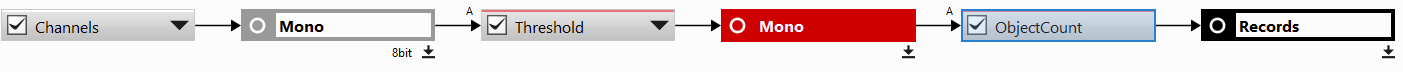
\includegraphics[width=0.75\textwidth]{artwork/simple-workflow.png}};
        % \draw[gray,very thin,step=1] (-5,-1) grid (5,1);
        \node (a) at (-5,-0.5){color};
        \node (b) at (-2,-0.5) {action};
        \node (c) at (0,-0.5) {binary};
        \node (d) at (4,-0.5) {table};
        \draw[->] (a) -| (-4,-0.2); 
        \draw[->] (b) -| (-1,-0.2); 
        \draw[->] (c) -| (1,-0.2); 
        \draw[->] (d) -| (5,-0.2); 
    \end{tikzpicture}
    \caption{A simple workflow with three kinds of nodes.}
    \label{fig:nodes}
\end{figure}

The recipes describes a workflow as a graph. The graph is compose of 4 types of nodes (See Fig.~\ref{fig:nodes}):
\begin{enumerate}\setlength\itemsep{0em}
    \item color: original or processed grayscale images
    \item action: processing steps on images, binary or tables
    \item binary: masks and labels
    \item results: tables with measurement results 
\end{enumerate}

To add an action, drag the new element to the previous one to automatically create a connection and keep the elements organized.

\paragraph{Storing results}

Saving of channels and binary layers can be enabled case by case using a right click on the layer. 

\subsection{Tips}
\begin{itemize}
    \item Use \keys{\Alt+\arrowkeyup} / \keys{\Alt+\arrowkeydown}  to increase / decrease the opacity of the binaries.
    \item To look for a module, use the search bar at the top.
    \item Right-click on the image and find image information for pixel to micron conversion.
    \item Click on the question mark on each operation (top left) for more information if needed.
\end{itemize}

\subsection{Image processing concepts}

\paragraph{Median filter} 

\paragraph{Rolling ball} Rolling ball is used for correcting shading and non-even background. It works by subtracting a background image estimated by dilating and eroding the image.

\paragraph{Watershed}

\paragraph{Thresholding}




